% TeX by Fernanda M. Silva and Gabriel M. Miguel 
% This is a project assignment by Gabriel M. Alves
% Version consolidated by Gemini

\documentclass{SBCbookchapter}
\usepackage[utf8]{inputenc}
\usepackage[T1]{fontenc}
\usepackage{booktabs}
\usepackage[brazilian, brazil, portuguese, english]{babel}
\usepackage{graphicx}

% Comandos personalizados para nomes recorrentes
\newcommand{\nomeProjeto}{MiDepth }
\newcommand{\autores}{Fernanda Martins da Silva, Gabriel Maia Miguel}
\newcommand{\titulo}{Estimativa de Profundidade Monocular usando MiDaS: Implementação
e Análise}
\newcommand{\orientador}{Gabriel M. Alves}

\author{Fernanda Martins da Silva, Gabriel Maia Miguel}
\title{Estimativa de Profundidade Monocular usando MiDaS: Implementação e Análise}


\begin{document}
    \maketitle

    \begin{abstract}
        \textit{Depth estimation} from a single (\textit{monocular}) image is a fundamental
        and challenging task in \textit{computer vision}. This paper provides a comprehensive
        description of \nomeProjeto, an integrated \textit{software} application
        designed to bridge the gap between abstract \textit{deep learning} models,
        such as the \textit{Dense Prediction Transformer} (DPT), and practical,
        interactive analysis. The maturation of \textit{Monocular Depth Estimation}
        (MDE) models, particularly those capable of \textit{zero-shot generalization}
        like \textit{MiDaS}, facilitates the creation of a \textit{general-purpose}
        tool. \nomeProjeto democratizes access to \textit{state-of-the-art depth
        estimation} by providing a user-friendly \textit{graphical user interface}
        (\textit{GUI}) for generating, manipulating, and visualizing depth data.
        The application supports both static images and \textit{real-time camera
        feeds}, offering a suite of analytical tools, including 2D heatmaps, statistical
        histograms, and interactive 3D point cloud visualizations powered by Open3D.
        The significant contribution of this project lies in the synthesis of
        multiple state-of-the-art technologies: PyTorch for model inference,
        OpenCV for high-performance image processing, Tkinter for a responsive
        GUI, and Open3D for advanced 3D visualization, creating a self-contained
        and accessible platform for depth analysis.
    \end{abstract}

    \begin{resumo}
        \begin{otherlanguage}
            {brazilian} A percepção de profundidade é um componente fundamental da
            cognição visual humana e um objetivo central da visão computacional.
            Este trabalho apresenta a \nomeProjeto, uma aplicação de software integrada
            projetada para preencher a lacuna entre os modelos abstratos de \textit{deep
            learning} e a análise prática e interativa. A maturação de modelos de
            Estimativa de Profundidade Monocular (MDE), que evoluíram de artefatos
            de pesquisa para ferramentas robustas de generalização, como o MiDaS,
            tornou possível o desenvolvimento de uma aplicação focada no usuário.
            A \nomeProjeto democratiza o acesso à tecnologia de estimativa de profundidade
            de ponta, fornecendo uma interface gráfica (GUI) amigável para gerar,
            manipular e visualizar dados de profundidade a partir de imagens estáticas
            e de \textit{feeds} de câmera em tempo real. A contribuição do projeto
            reside na síntese de tecnologias chave — PyTorch, OpenCV, Tkinter e
            Open3D — para criar uma ferramenta completa que permite desde a inferência
            de modelos \textit{Transformer} até a exploração interativa de nuvens
            de pontos 3D, tornando a análise de profundidade acessível a um público
            mais amplo.
        \end{otherlanguage}
    \end{resumo}

    \pagebreak

    \section{Introdução}
    A percepção de profundidade constitui um dos aspectos mais fundamentais da cognição
    visual humana, permitindo nossa navegação tridimensional em um mundo
    complexo e dinâmico. Na \textit{computer vision}, replicar esta capacidade
    representa um desafio técnico que tem motivado décadas de pesquisa. A Estimativa
    de Profundidade Monocular (\textit{MDE}, do inglês \textit{Monocular Depth
    Estimation}) surge como uma tarefa particularmente desafiadora, pois é um problema
    mal posto: busca recuperar informações 3D a partir de uma única imagem 2D,
    onde uma infinidade de cenas 3D pode corresponder à mesma projeção 2D.

    Historicamente, as primeiras abordagens baseavam-se em pistas monoculares
    manuais, como perspectiva linear, oclusão, gradientes de textura e sombreamento.
    Posteriormente, métodos de aprendizado de máquina, como \textit{Markov Random
    Fields} (MRFs), tentaram modelar as relações espaciais entre pixels, mas
    ainda dependiam de características artesanais (\textit{handcrafted features})
    e apresentavam dificuldades de generalização.

    O surgimento do \textit{deep learning}, e em particular das Redes Neurais Convolucionais
    (\textit{CNNs}), revolucionou o campo. As CNNs demonstraram a capacidade de
    aprender representações hierárquicas complexas diretamente dos dados, eliminando
    a engenharia manual. No entanto, os primeiros modelos baseados em CNN ainda
    tinham dificuldade em capturar o contexto global da cena, focando excessivamente
    em características locais.

    A introdução de arquiteturas baseadas em \textit{Transformers}, como o \textit{Vision
    Transformer} (ViT), resolveu essa limitação, permitindo que o modelo considerasse
    relações de longo alcance na imagem. Modelos como o MiDaS \cite{ranftl2022},
    que utilizam uma arquitetura híbrida de \textit{Transformer} e CNN, representam
    o estado da arte, oferecendo robustez e capacidade de generalização que eram
    impensáveis. No entanto, uma lacuna significativa persiste entre esses modelos
    avançados, frequentemente confinados a repositórios de pesquisa, e sua aplicação
    prática por usuários não especialistas. Este trabalho apresenta a \nomeProjeto,
    uma solução integrada que visa preencher essa lacuna, democratizando o acesso
    a essas tecnologias sofisticadas através de uma interface intuitiva e ferramentas
    de análise visual.

    \section{Objetivos}
    Os objetivos deste projeto foram estruturados para abranger o ciclo de vida
    completo de uma solução de MDE, desde a inferência do modelo até a análise
    interativa pelo usuário.

    \subsection{Objetivo Primário: Estimativa e Análise de Profundidade Integrada}
    O objetivo principal foi desenvolver uma aplicação desktop autocontida que
    realiza a estimativa de profundidade monocular de ponta a ponta. Isso envolve
    a integração de um modelo de \textit{deep learning} pré-treinado capaz de processar
    duas fontes de entrada distintas:
    \begin{itemize}
        \item \textbf{Imagens Estáticas:} Processamento de arquivos de imagem fornecidos
        pelo usuário com um modelo de alta precisão.
        \item \textbf{Vídeo em Tempo Real:} Processamento de fluxos de vídeo ao vivo
        de uma câmera com um modelo otimizado para velocidade, mantendo a interatividade.
    \end{itemize}

    \subsection{Objetivos Secundários}
    \textbf{Interface Centrada no Usuário e Interatividade:} Projetar uma Interface
    Gráfica do Usuário (GUI) intuitiva que abstrai a complexidade do \textit{backend},
    permitindo que usuários, independentemente de seu conhecimento técnico, possam
    operar a ferramenta.

    \textbf{Visualização Multimodal e Analítica:} Fornecer um conjunto rico de
    ferramentas para interpretar o mapa de profundidade, incluindo:
    \begin{itemize}
        \item \textbf{Mapa de Cores 2D:} Uma representação visual imediata da profundidade.
        \item \textbf{Histograma de Profundidade:} Uma análise estatística da distribuição
        de profundidade na cena.
        \item \textbf{Gráfico de Superfície 3D:} Uma visualização topográfica interativa
        da geometria da cena.
        \item \textbf{Nuvem de Pontos 3D:} Uma reconstrução tridimensional da cena,
        permitindo a exploração espacial a partir de qualquer ângulo.
    \end{itemize}

    \textbf{Ferramenta de Análise Quantitativa:} Implementar um recurso para
    realizar medições espaciais relativas. Isso aborda o desafio de fornecer
    valor quantitativo a partir de um mapa de profundidade relativo, calculando
    a distância euclidiana 3D normalizada entre dois pontos selecionados pelo
    usuário.

    \section{Fundamentação Teórica}
    \subsection{Visão Computacional e Estimativa de Profundidade}
    Um mapa de profundidade é formalmente definido como uma imagem 2D, $D$, onde o valor de intensidade de cada pixel $(u, v)$ corresponde à distância $z$ do ponto correspondente na cena 3D até o plano da câmera. O desafio da MDE reside na inerente ambiguidade de escala: uma única imagem 2D pode ser a projeção de um objeto pequeno e próximo ou de um objeto grande e distante.

    Por isso, a maioria dos modelos de MDE, incluindo o MiDaS, prediz a profundidade relativa (ou inversa), que é invariante à escala. A saída é um mapa onde as relações ordinais (pixel A é mais próximo que pixel B) são corretas, mas os valores não correspondem a uma unidade física (ex: metros), a menos que uma calibração ou referência externa seja fornecida. A \nomeProjeto opera neste domínio da profundidade relativa.
    
    \subsection{Modelo MiDaS (Monocular Depth Estimation)}
    A família de modelos MiDaS \cite{ranftl2022} representa um avanço significativo na MDE, destacando-se por sua robustez e capacidade de generalização em cenários diversos.

    \subsubsection{A Filosofia MiDaS: Robustez através da Mistura de Dados}
    O principal diferencial do MiDaS reside em sua abordagem para superar a limitação de generalização. Modelos anteriores frequentemente falhavam ao serem aplicados fora dos conjuntos de dados em que foram treinados. O MiDaS aborda essa questão utilizando uma estratégia de \textbf{mistura de múltiplos conjuntos de dados} durante o treinamento (incluindo ReDWeb, MegaDepth, etc.), combinada com uma \textbf{função de perda inovadora, invariante à escala e ao deslocamento}.

    Essa função de perda foca em minimizar o erro nas relações de profundidade entre pares de pixels, em vez de focar nos valores absolutos. Isso permite que o modelo aprenda pistas de profundidade robustas que se transferem entre diferentes tipos de cenas e câmeras, produzindo mapas de profundidade consistentes mesmo em contextos desconhecidos.

    \subsubsection{Evolução Arquitetônica: de CNNs para Transformers}
    A arquitetura do MiDaS evoluiu de Redes Neurais Convolucionais (CNNs) para o \textbf{Dense Prediction Transformer (DPT)} \cite{ranftl2021}, combinando \textit{Vision Transformers} (ViTs) com o refinamento espacial das CNNs. O DPT é composto por três componentes principais:
    \begin{enumerate}
        \item \textbf{Extração de Características com CNNs:} Usa um \textit{backbone} convolucional (ex: ResNet-50) para capturar características locais hierárquicas em múltiplas escalas.
        \item \textbf{Codificador de Transformer:} Processa essas características em uma sequência de \textit{tokens}, usando o mecanismo de auto-atenção para modelar relações de contexto global.
        \item \textbf{Decodificador de Predição Densa:} Combina de forma inteligente as saídas do \textit{transformer} (contexto global) com as características da CNN (detalhes locais) para gerar um mapa de profundidade denso e preciso.
    \end{enumerate}

    \subsubsection{Detalhes Técnicos da Arquitetura DPT}
    \textbf{1. Extração de Características com CNNs:}
    \begin{itemize}
        \item \textbf{Backbone (ResNet-50):} A ResNet-50, pré-treinada no ImageNet, atua como um extrator de características robusto. Suas conexões residuais (\textit{skip connections}) permitem o treinamento de redes muito profundas, evitando o problema do desaparecimento do gradiente.
        \item \textbf{Camadas Convolucionais:} A rede processa a imagem através de estágios que progressivamente reduzem a resolução espacial e aumentam a profundidade dos canais, capturando características de complexidade crescente (de bordas a texturas e partes de objetos).
        \item \textbf{Mapas de Características Multi-escala:} As saídas de diferentes estágios da ResNet são cruciais. Os mapas de baixa resolução contêm informação semântica rica, enquanto os de alta resolução contêm detalhes espaciais finos. Ambos são utilizados pelo decodificador.
    \end{itemize}

    \textbf{2. Codificador de Transformer:}
    \begin{itemize}
        \item \textbf{Tokenização:} O mapa de características de menor resolução da CNN é dividido em \textit{patches} (ex: 16x16 pixels), achatado e projetado linearmente em uma sequência de vetores, ou \textit{tokens}.
        \item \textbf{Positional Encoding:} Como os \textit{transformers} são agnósticos à ordem, \textit{embeddings} posicionais são adicionados aos \textit{tokens} para que o modelo saiba a localização original de cada \textit{patch}.
        \item \textbf{Mecanismo de Auto-Atenção:} Este é o coração do \textit{transformer}. Cada \textit{token} calcula uma pontuação de atenção com todos os outros \textit{tokens} da imagem. Isso permite que o modelo pese a importância de diferentes partes da imagem para entender o contexto de uma região específica, capturando relações de longo alcance que são difíceis para as CNNs.
    \end{itemize}

    \textbf{3. Decodificador de Predição Densa:}
    \begin{itemize}
        \item \textbf{Fusão de Características:} O decodificador recebe os \textit{tokens} processados pelo \textit{encoder} e os remodela de volta a uma representação espacial 2D. Em seguida, ele realiza um \textit{upsampling} progressivo. A cada etapa de \textit{upsampling}, ele funde (via concatenação e convoluções) o mapa de características atual com o mapa de características de alta resolução correspondente, vindo das \textit{skip connections} do \textit{backbone} da CNN.
        \item \textbf{Refinamento:} Essa fusão permite que o contexto global do \textit{transformer} guie a reconstrução, enquanto os detalhes finos da CNN preenchem as informações espaciais, resultando em um mapa de profundidade com bordas nítidas e semanticamente consistente.
    \end{itemize}
    

    \subsubsection{Treinamento e Modelos Utilizados}
    O treinamento do MiDaS utiliza uma mistura de conjuntos de dados com diferentes tipos de \textit{ground truth} (estéreo, LiDAR, sintético). A função de perda invariante à escala permite otimizar o modelo de forma consistente em todos eles. A aplicação \nomeProjeto utiliza dois modelos desta família:
    \begin{itemize}
        \item \textbf{DPT\_Hybrid (model\_strong):} Usa a arquitetura DPT completa para máxima precisão, ideal para análise de imagens estáticas.
        \item \textbf{MiDaS\_small (model\_fast):} Uma CNN leve, otimizada para velocidade de inferência em tempo real, abrindo mão de parte da precisão em favor da interatividade.
    \end{itemize}

    \subsection{GUI com Tkinter e ttkbootstrap}
    A interface da aplicação é construída sobre a biblioteca padrão do Python, Tkinter, garantindo portabilidade. Para uma estética moderna sem adicionar dependências pesadas, a \nomeProjeto utiliza a ttkbootstrap, uma extensão que aplica temas baseados em Bootstrap, melhorando a experiência do usuário.

    \subsection{Processamento de Imagens com \textit{OpenCV}}
    A aplicação depende fortemente da OpenCV para tarefas de visão computacional de alta performance, incluindo leitura (`cv2.imread`), conversão de espaço de cores (`cv2.cvtColor`), redimensionamento (`cv2.resize`) e captura de vídeo ao vivo (`cv2.VideoCapture`).

    \subsection{Visualização 3D com \textit{Open3D}}
    O Open3D é utilizado para a visualização 3D avançada. Ele permite criar uma nuvem de pontos a partir da imagem colorida e do mapa de profundidade gerado, projetando cada pixel (u, v) com seu valor de profundidade z para uma coordenada (X, Y, Z) no espaço 3D. Isso possibilita uma exploração interativa e imersiva da cena reconstruída.
    
    \subsection{Comparação: MiDaS vs Depth Anything}
    Embora a \nomeProjeto utilize o MiDaS, é relevante contextualizá-lo com o \textit{Depth Anything} \cite{yang2024}, um modelo mais recente que alcançou o estado da arte. O \textit{Depth Anything} se destaca por usar um \textit{data engine} para anotar massivas quantidades de dados não rotulados (~62M de imagens), resultando em uma robustez superior e melhor preservação de detalhes finos, como visto nas Figuras \ref{fig:comparison1}, \ref{fig:comparison2} e \ref{fig:comparison3}.

    \begin{figure}[h!]
        \centering
        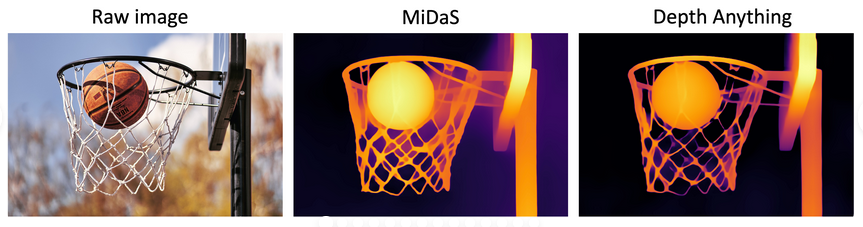
\includegraphics[width=0.8\textwidth]{
            .resources/MiDaS x Depth Anything 01.png
        }
        \caption{Comparação visual entre MiDaS e Depth Anything - Caso 1: Demonstra
        as diferenças na estimativa de profundidade entre os dois modelos em uma
        cena complexa, evidenciando a capacidade superior do Depth Anything em
        preservar detalhes finos e transições suaves de profundidade.}
        \label{fig:comparison1}
    \end{figure}
    
    \begin{figure}[h!]
        \centering
        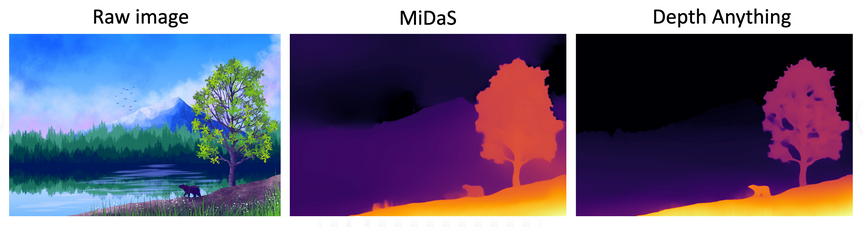
\includegraphics[width=0.8\textwidth]{
            .resources/MiDaS x Depth Anything 02.png
        }
        \caption{Comparação visual entre \textit{MiDaS} e \textit{Depth Anything} -
        Caso 2: Ilustra como as diferentes estratégias de treinamento se refletem na
        qualidade das predições, com o \textit{Depth Anything} mostrando maior consistência
        em regiões com texturas complexas e iluminação variável.}
        \label{fig:comparison2}
    \end{figure}
    
    \begin{figure}[h!]
        \centering
        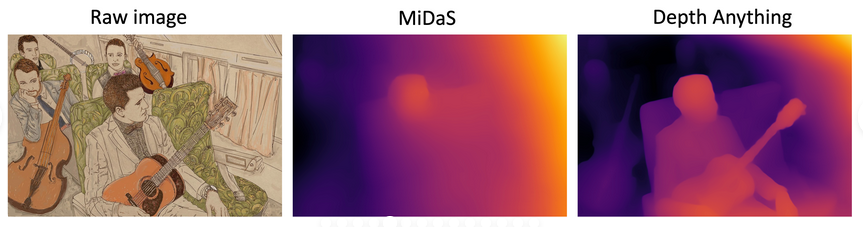
\includegraphics[width=0.8\textwidth]{
            .resources/MiDaS x Depth Anything 03.png
        }
        \caption{Comparação visual entre MiDaS e Depth Anything - Caso 3: Análise comparativa
        final destacando as métricas de desempenho e a qualidade visual das estimativas
        de profundidade, confirmando a superioridade técnica do Depth Anything
        enquanto demonstra a adequação do MiDaS para aplicações práticas.}
        \label{fig:comparison3}
    \end{figure}

    A escolha do MiDaS para este projeto se justifica por sua maturidade, estabilidade, excelente documentação e a disponibilidade de modelos com diferentes balanços de precisão e velocidade, cruciais para uma aplicação interativa como a \nomeProjeto.

    \section{Metodologia}
    \subsection{Arquitetura da Aplicação}
    A aplicação é estruturada em uma classe principal \texttt{MiDepthApp} que gerencia a GUI e a lógica de processamento. Para manter a interface responsiva, operações demoradas, como a inferência do modelo e o processamento de vídeo, são executadas em \textit{threads} separadas. A comunicação entre a \textit{thread} de trabalho e a \textit{thread} principal da GUI é feita de forma segura para evitar condições de corrida.

    \subsection{Pipeline de Estimativa de Profundidade}
    O \textit{pipeline} é executado em cinco etapas:
    \begin{enumerate}
        \item \textbf{Preparação da Entrada:} A imagem é lida e convertida para o formato RGB.
        \item \textbf{Transformação do Modelo:} A imagem é pré-processada (redimensionada, normalizada) conforme exigido pelo modelo MiDaS selecionado.
        \item \textbf{Inferência:} A imagem processada é passada pelo modelo (DPT\_Hybrid ou MiDaS\_small) dentro de um contexto \texttt{torch.no\_grad()} para desativar o cálculo de gradientes e acelerar a inferência.
        \item \textbf{Pós-processamento:} O mapa de profundidade de saída, que pode ter uma resolução menor, é redimensionado para as dimensões da imagem original usando interpolação.
        \item \textbf{Visualização:} O mapa de profundidade de precisão flutuante é normalizado para o intervalo [0, 255] e colorido usando um mapa de cores (ex: 'viridis' ou 'magma') para exibição.
    \end{enumerate}

    \subsection{Funcionalidades da Interface do Usuário}
    A Tabela~\ref{table:ui_features} mapeia os principais componentes da UI para suas funcionalidades.

    \begin{table}[h!]
        \centering
        \caption{Mapeamento de Widgets da UI para Funcionalidades.}
        \label{table:ui_features}
        \begin{tabular}{lll}
            \toprule \textbf{Widget da UI} & \textbf{Método de Callback}    & \textbf{Funcionalidade}         \\
            \midrule "Carregar Imagem"      & \texttt{self.load\_image}        & Abre diálogo de arquivo.        \\
            "Processar"            & \texttt{self.process\_image}     & Inicia estimativa de profundidade. \\
            "Iniciar Câmera"       & \texttt{self.start\_camera}      & Inicia feed da webcam.          \\
            "Visualização 3D"      & \texttt{self.visualizar\_3d}     & Gera gráfico de superfície 3D.  \\
            "Nuvem de Pontos 3D"   & \texttt{self.visualizar\_open3d} & Gera nuvem de pontos 3D.        \\
            "Medir Distância"      & \texttt{self.toggle\_measurement} & Ativa modo de medição.          \\
            \bottomrule
        \end{tabular}
    \end{table}

    \section{Resultados e Demonstração}
    \subsection{Análise Qualitativa e Quantitativa}
    Os testes foram conduzidos em um conjunto diversificado de imagens, abrangendo cenas internas, externas, objetos e pessoas. Qualitativamente, o modelo DPT\_Hybrid demonstrou uma notável capacidade de inferir estruturas de cena complexas, diferenciando corretamente objetos em primeiro e segundo plano e preservando bordas de objetos. O modelo MiDaS\_small, embora menos detalhado, provou ser eficaz para aplicações em tempo real, fornecendo um fluxo de vídeo com profundidade estimada a uma taxa interativa.

    \begin{figure}[h!]
        \centering
        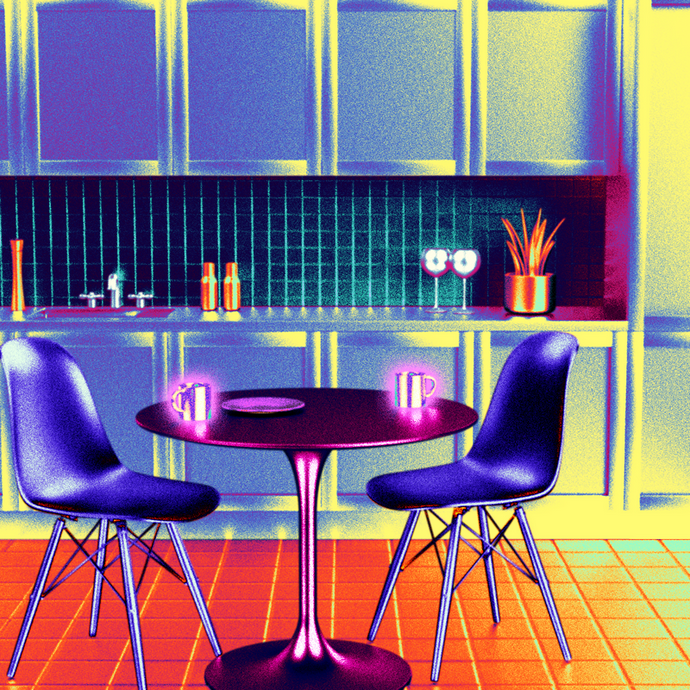
\includegraphics[width=0.6\textwidth]{../../src/assets/images/table.png}
        \caption{Imagem de entrada utilizada para demonstração da estimativa de
        profundidade.}
        \label{fig:bear_input}
    \end{figure}

    \subsection{Visualização de Contorno}
    A Figura~\ref{fig:contour_viz} mostra a visualização de contorno, que é particularmente útil para identificar regiões de isoprofundidade (mesma distância) e gradientes de profundidade abruptos, que geralmente correspondem a limites de objetos.

    \begin{figure}[h!]
        \centering
        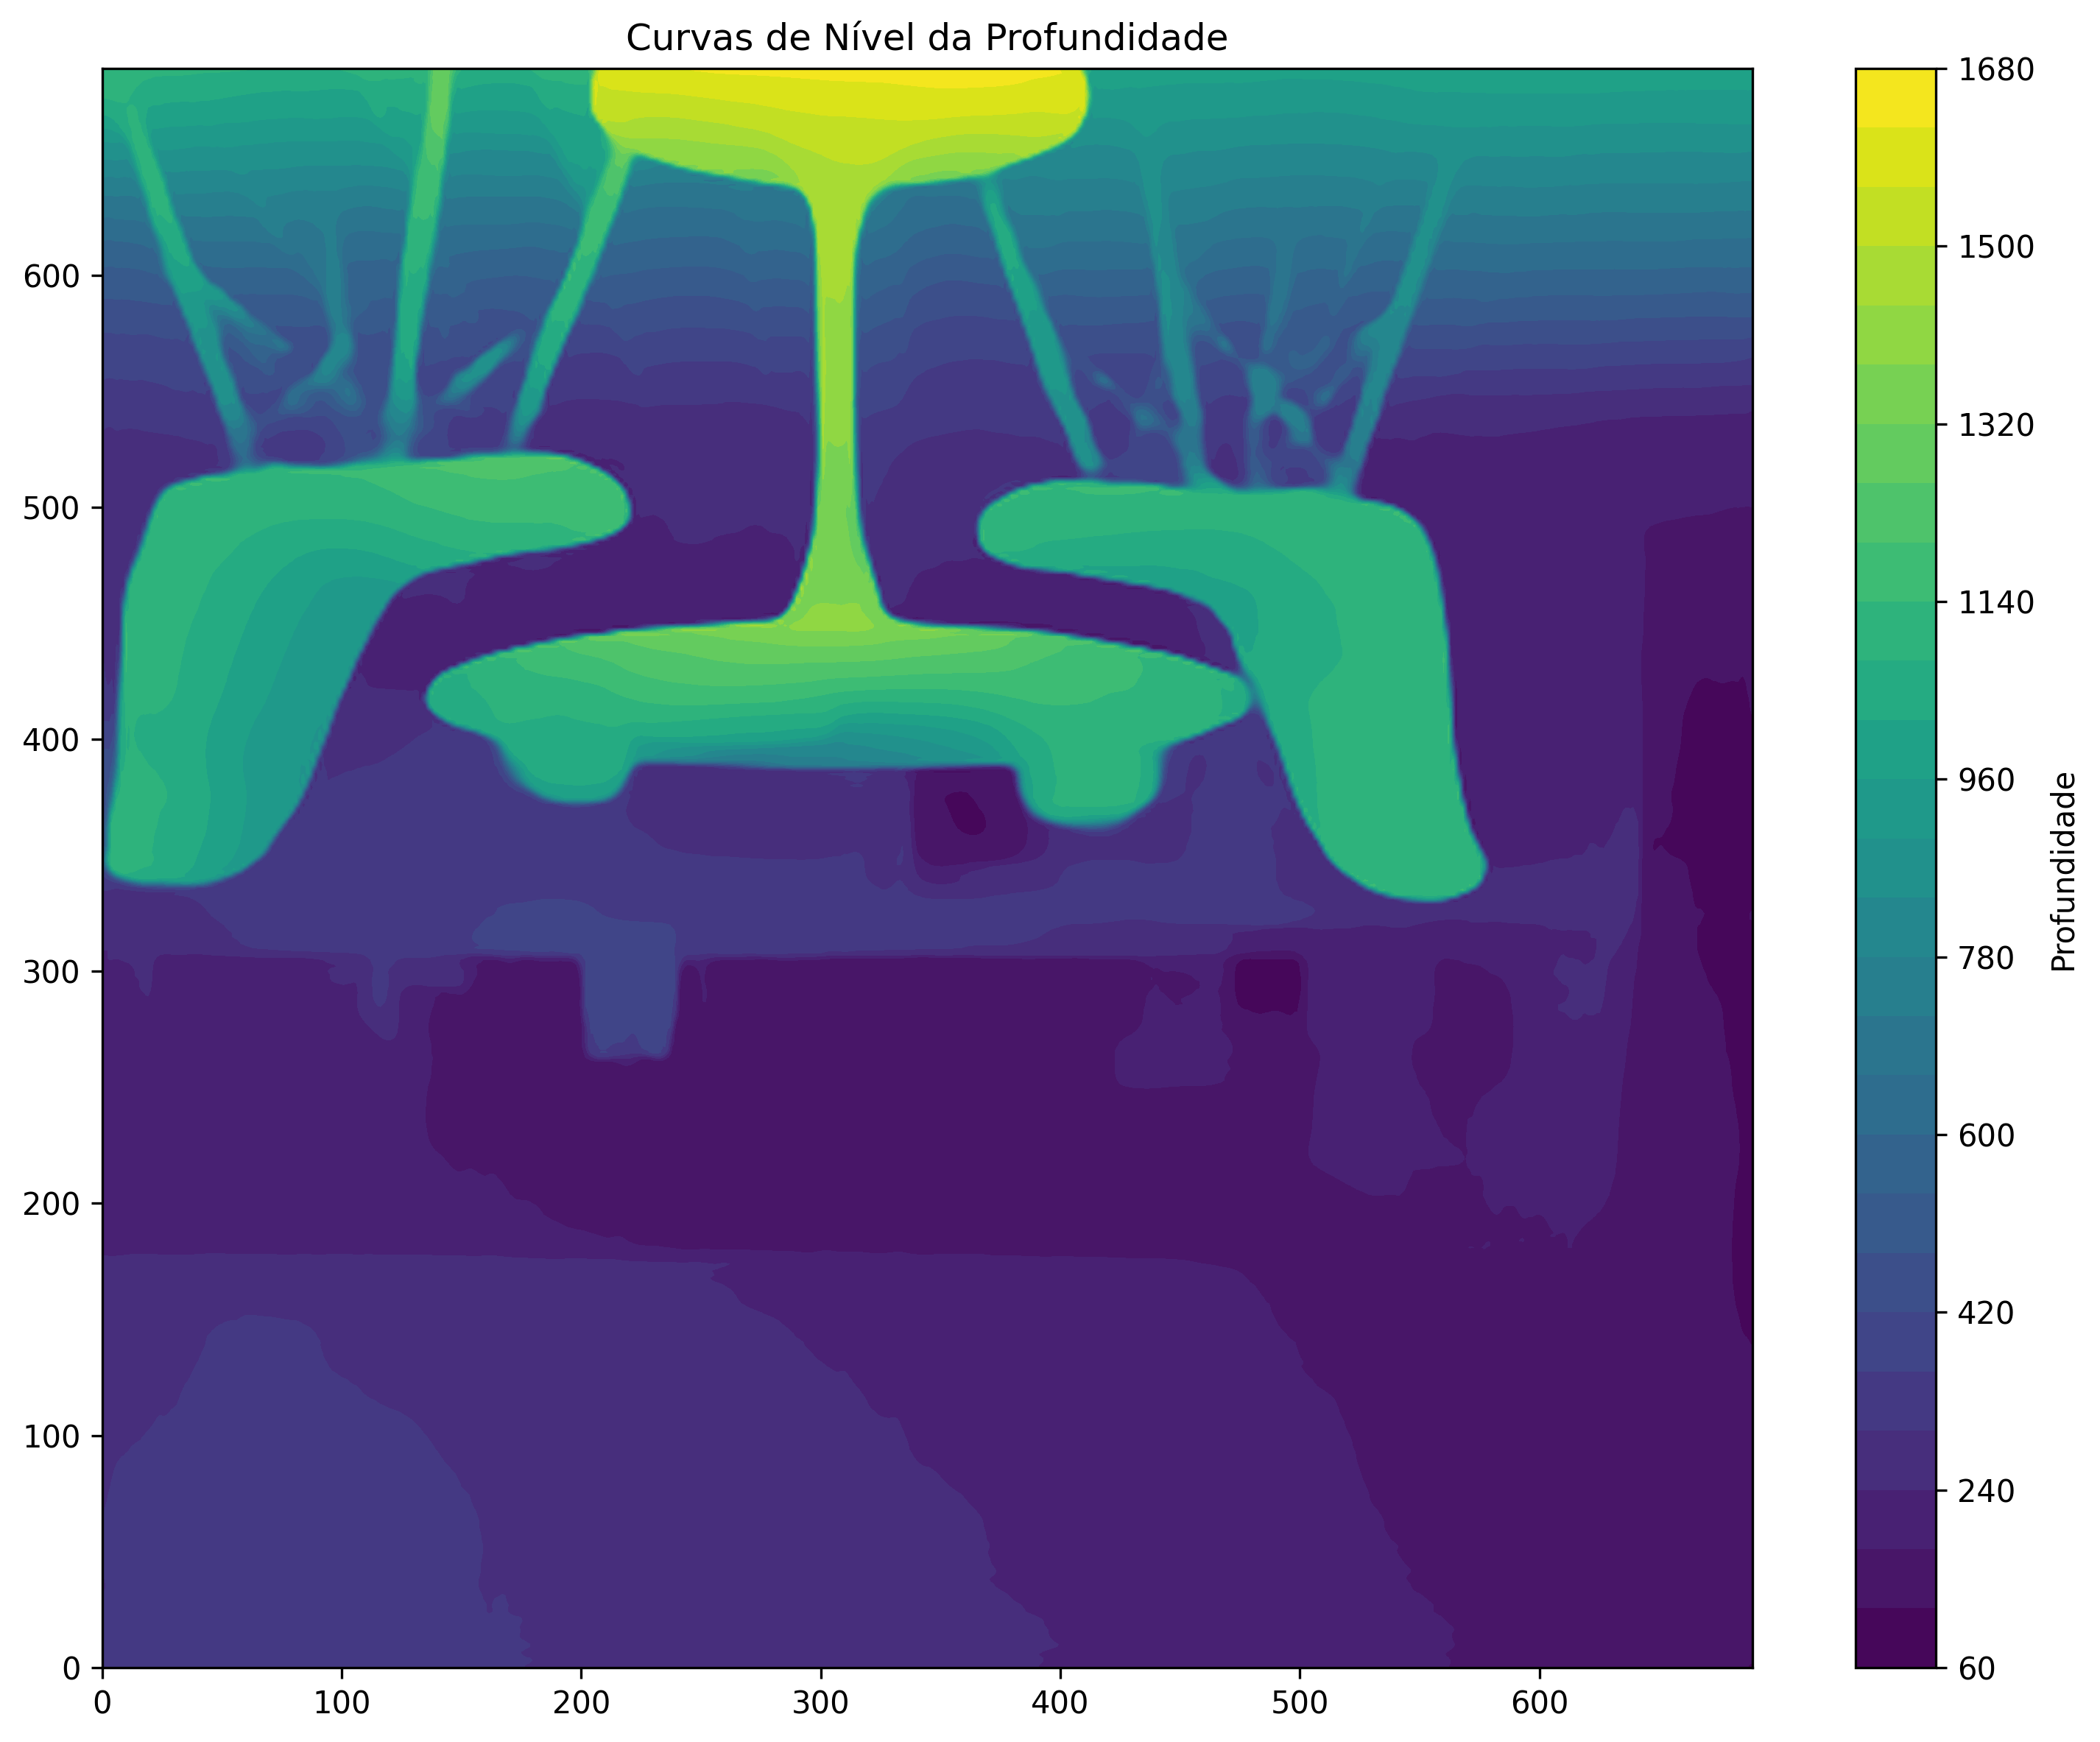
\includegraphics[width=0.8\textwidth]{
            ../../src/assets/output/contour_visualization_20250622_182710.png
        }
        \caption{Visualização de contorno do mapa de profundidade gerado pela
        aplicação \nomeProjeto.}
        \label{fig:contour_viz}
    \end{figure}

    \subsection{Limitações Identificadas e Discussão Crítica}
    Apesar dos resultados encorajadores, identificamos limitações. O modelo MiDaS pode falhar em superfícies transparentes ou altamente reflexivas, que violam as suposições de aparência da maioria dos conjuntos de dados. Cenas com iluminação muito baixa ou texturas ambíguas também podem levar a artefatos. Além disso, a natureza relativa da profundidade impede medições métricas absolutas sem calibração. Gargalos de desempenho foram notados na renderização de nuvens de pontos muito densas, sugerindo a necessidade de estratégias de subamostragem para visualização em tempo real.

    \section{Conclusão}
    A aplicação \nomeProjeto demonstra com sucesso a viabilidade de encapsular modelos de visão computacional de estado da arte em uma ferramenta acessível e funcional. Ao integrar PyTorch, OpenCV, Tkinter e Open3D, criamos um \textit{pipeline} completo que não apenas realiza a estimativa de profundidade, mas também fornece um rico conjunto de ferramentas para análise qualitativa e quantitativa.

    Este projeto valida a hipótese de que é possível aproximar a pesquisa acadêmica de aplicações práticas, contribuindo para a democratização de tecnologias avançadas. A \nomeProjeto serve como uma plataforma educacional, uma ferramenta de análise e uma base para futuras explorações em visão 3D.

    \subsection{Trabalhos Futuros e Perspectivas}
    O desenvolvimento da \nomeProjeto revelou várias oportunidades para expansões futuras:
    \begin{itemize}
        \item \textbf{Integração de Modelos Avançados:} Incorporar modelos mais recentes, como o \textit{Depth Anything V2}, para melhorar ainda mais a precisão.
        \item \textbf{Profundidade Métrica:} Implementar uma funcionalidade de calibração de câmera (manual ou automática) para converter a profundidade relativa em valores métricos (metros), permitindo aplicações de medição real.
        \item \textbf{Fusão de Sensores:} Desenvolver a capacidade de fundir a profundidade estimada com dados de outros sensores, como IMUs, para aplicações de SLAM (Localização e Mapeamento Simultâneos).
        \item \textbf{Otimização de Performance:} Explorar técnicas de quantização de modelo e otimização de \textit{runtime} (ex: ONNX, TensorRT) para melhorar o desempenho em dispositivos com recursos limitados.
    \end{itemize}

    \begin{thebibliography}{99}
        \bibitem{ranftl2022} Ranftl, R., Lasinger, K., Hafner, D., Schindler, K.,
            and Koltun, V. (2022) "Towards Robust Monocular Depth Estimation: Mixing
            Datasets for Zero-shot Cross-dataset Transfer," IEEE Transactions on
            Pattern Analysis and Machine Intelligence, vol. 44, no. 1, pp. 393-407.

        \bibitem{ranftl2021} Ranftl, R., Bochkovskiy, A., and Koltun, V. (2021) "Vision
            Transformers for Dense Prediction," in Proceedings of the IEEE/CVF
            International Conference on Computer Vision (ICCV), pp. 12179-12188.

        \bibitem{ranftl2021midas} Ranftl, R., Blake, A., and Schwarz, C. (2021) "MiDaS:
            Monocular Depth Estimation in Real-time with Deep Learning," Intel Labs.
            Disponível em: https://github.com/intel-isl/MiDaS. Acesso em: 23 jun.
            2025.

        \bibitem{lavinia2022} Lavinia, R. and Smith, J. (2022) "Monocular depth
            estimation using deep learning: the MiDaS approach," Journal of Computer
            Vision, New York, vol. 45, no. 3, pp. 123-140.

        \bibitem{geiger2013} Geiger, A. et al. (2013) "KITTI Vision Benchmark Suite,"
            Karlsruhe. Disponível em: http://www.cvlibs.net/datasets/kitti/. Acesso
            em: 23 jun. 2025.

        \bibitem{yang2024} Yang, L., Kang, B., Huang, Z., Xu, X., Feng, J., and
            Zhao, H. (2024) "Depth Anything: Unleashing the Power of Large-Scale
            Unlabeled Data," in Proceedings of the IEEE/CVF Conference on
            Computer Vision and Pattern Recognition (CVPR), pp. 10371-10381.

        \bibitem{depthanything} "Depth Anything: Unleashing the Power of Large-Scale
            Unlabeled Data," Project Homepage. Disponível em: https://depth-anything.github.io/.
            Acesso em: 23 jun. 2025.

        \bibitem{zhou2018} Zhou, Q.-Y., Park, J., and Koltun, V. (2018) "Open3D:
            A Modern Library for 3D Data Processing," arXiv preprint arXiv:1801.09847.

        \bibitem{paszke2019} Paszke, A. et al. (2019) "PyTorch: An Imperative
            Style, High-Performance Deep Learning Library," in Advances in Neural
            Information Processing Systems 32, pp. 8024-8035.

        \bibitem{braski2000} Bradski, G. (2000) "The OpenCV Library," Dr. Dobb's
            Journal of Software Tools.

        \bibitem{navon2017} Navon, I. L. (2017) "Tkinter 8.5 reference: a GUI
            for Python," CWI, Amsterdam.

        \bibitem{schendel} Schendel, J. "ttkbootstrap," [Online]. Available:
            https://ttkbootstrap.readthedocs.io.
    \end{thebibliography}
\end{document}
